\documentclass[a4paper, 12pt, titlepage]{article}

\usepackage[utf8]{inputenc}
\usepackage{geometry}
\usepackage{polski}
\usepackage{graphicx} 
\usepackage{float} 
\usepackage{etoolbox,refcount}
\usepackage{multicol}
\usepackage{fancyhdr}
\usepackage{listings}
\usepackage{amsmath}
\usepackage{tabularx}

\pdfsuppresswarningpagegroup=1
\newgeometry{left=2.5cm, right=2.5cm, bottom=2.5cm, top=2.5cm}

\lstset{
    language=Matlab,
    basicstyle=\ttfamily,
    keepspaces=true,
    frame=single,
    tabsize=4,
    showspaces=false,
    showstringspaces=false,
    extendedchars=true,
    inputencoding=utf8,
    literate={ó}{{\'o}}1 {ę}{{\k{e}}}1 {ł}{{\l{}}}1 {ż}{{\.z}}1
        {ś}{{\'s}}1 {ć}{{\'c}}1 {ą}{{\k{a}}}1 {ź}{{\'z}}1 {ń}{{\'n}}1
}

\author{Adrian Jałoszewski}
\title{Ćwiczenie 5: AUDIO -- analiza sygnału mowy}
\date{4 listopada 2017}

\begin{document}
    \maketitle
    \section{Parametry sygnału z ćw. 1} 
        \begin{figure}[H]
            \centering
            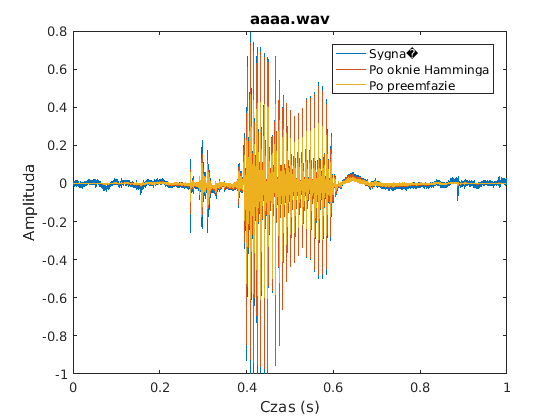
\includegraphics[width=0.8\linewidth]{Hamming.png}
            \caption{Kroki preprocessingu sygnału}
        \end{figure}
        \begin{figure}[H]
            \centering
            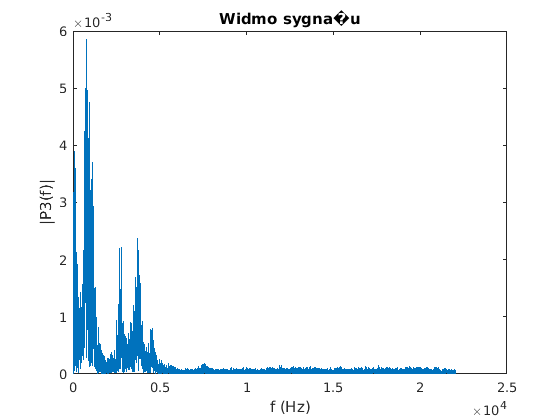
\includegraphics[width=0.8\linewidth]{FFT.png}
            \caption{Transformata Fouriera sygnału}
        \end{figure}
        \begin{figure}[H]
            \centering
            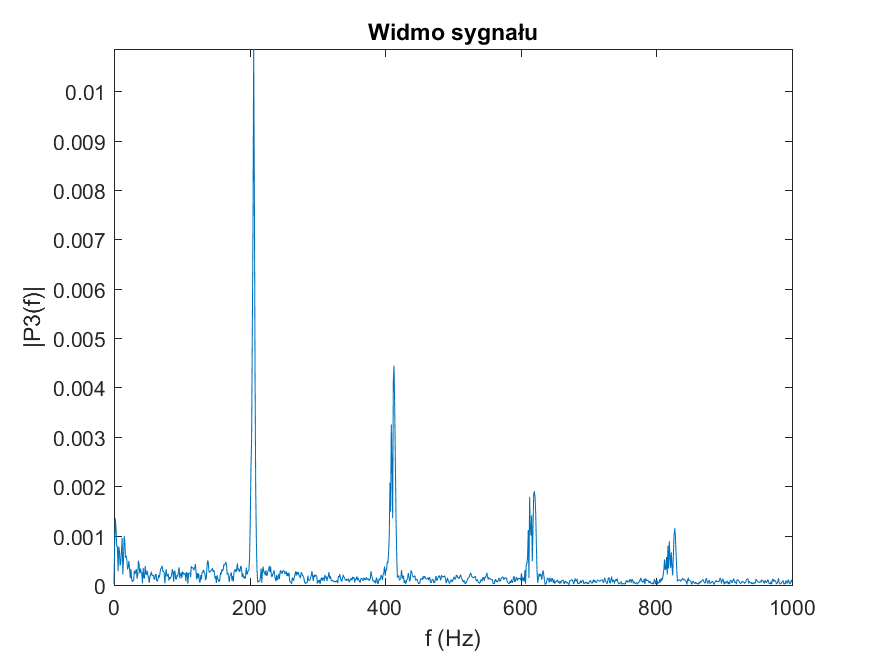
\includegraphics[width=0.8\linewidth]{FFT_2.png}
            \caption{Przybliżenie na harmoniczne}
        \end{figure}
        Po dłuższym zastanowieniu można zauważyć, że w skrypcie
        odpowiedzialnym za dokonanie analizy sygnału filtr jest
        ustawiony odwrotnie i dokonuje deemfazy zamiast preemfazy.
        Toteż w miejscu, gdzie jest tu sygnał poddany preemfazie 
        powinien znajdować się sygnał deemfazy (przynajmniej
        zgodnie z innymi źródłami znalezionymi w internecie).
        Błąd polega na tym, że w skrypcie licznik jest zamieniony
        z mianownikiem -- jest to deemfaza.
        \begin{itemize}
            \item[--] $F_1$ = 207.5 Hz, $F_2$ =416 Hz, $F_3$ = 620 Hz
            \item[--] $T$ = 4.83ms
        \end{itemize}
        Wartości te są powiązane tak, że pierwsza harmoniczna jest
        równa odwrotności okresu, a druga i trzecia są pierwszą 
        harmoniczną przemnożoną odpowiednio przez 2 i 3.
    \section{Okna czasowe dla sygnałów dyskretnych}
        Podczas analizy sygnału analogowego metodą DFT występuje zjawisko
        przecieku. Okna czasowe są wykorzystywane do jego minimalizacji.
        Zjawisko przecieku polega na tym, że w przypadku braku próbkowania
        z częstotliwościami występującymi w sygnale, to rozkłada się na
        częstotliwości występujące w FFT. Dzięki stosowaniu okien czasowych
        można ograniczyć zjawisko przecieku bez konieczności poszerzania okna.

        Zastosowanie okien może jednak spowodować utratę informacji
        (wycinany jest fragment historii sygnału).
    \section{Filtr preemfazy}
        Preemfaza jest używana aby uniezależnić sygnał od szumu. Szum ma zwykle
        duże częstotliwości, dlatego też składowe o wyższych częstotliwościach 
        mają wzmacnianą amplitudę -- oddziela się je od szumów. 
        \\ \\
        Przeciwieństwem preemfazy jest deemfaza -- jak już mamy do czynienia z 
        dalszym przetwarzaniem sygnału można cofnąć efekt preemfazy.
    \section{Tabela oraz formanty w przestrzeni formantów F1-F2-F3}
        Pierwsze trzy formanty sygnału pobranego:
        $$
            987.55\mathrm{Hz}, \mathrm{1945.09Hz}, \mathrm{2955.24Hz}
        $$
        \textbf{Formanty są niepowiązane z harmonicznymi sygnału}. Formant 
        jest pasmem częstotliwości dla których częstotliwości składowe
        ulegają szczególnemu wzmocnieniu.
        \\ \\
        Poniższe dane są uzyskane na podstawie danych w pełni uzyskanych
        od innych osób, ponieważ na stanowisku były problemy z kartą
        dźwiękową. Na poniższym wykresie dane uśrednione zaznaczone są 
        kółkiem, a kropkami oznaczone są poszczególne punkty pomiarowe.
        \begin{figure}[H]
            \centering
            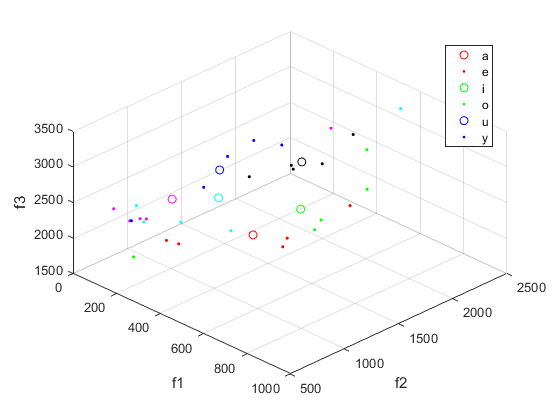
\includegraphics[width=0.8\linewidth]{clusters_correct.png}
            \caption{Formanty w przestrzeni F1-F2-F3 oraz średnie dla
                samogłosek}
        \end{figure}
        Legenda na wykresie jest niepoprawna (zauważone po wykonaniu
        laboratorium).
        \begin{itemize}
            \item[--] a -- czerwony
            \item[--] e -- zielony
            \item[--] i -- niebieski
            \item[--] o -- cyjan
            \item[--] u -- magenta
            \item[--] y -- czarny
        \end{itemize}
        \begin{table}[H]
            \centering
            \caption{Formanty dla samogłosek}
            \begin{tabular}{|l|l|r|r|r|}
                \hline
                 & Class & F1 & F2 & F3 \\ \hline 
                a\_1\_jp & 'a' & 676.83 & 1079.9 & 2423.2 \\ \hline
                a\_1\_mjk & 'a' & 669.95 & 1134.8 & 2497 \\ \hline
                a\_1\_mrjs & 'a' & 216.73 & 1040.9 & 1841.6 \\ \hline
                a\_2\_mrjs & 'a' & 867.67 & 1318 & 3105.3 \\ \hline
                a\_3\_mrjs & 'a' & 174.71 & 1012.1 & 1851.7 \\ \hline
                e\_1\_jp & 'e' & 581.19 & 1564.5 & 2184.6 \\ \hline
                e\_1\_mjk & 'e' & 581.5 & 1623.4 & 2282 \\ \hline
                e\_1\_mrjs & 'e' & 677.19 & 1855.8 & 2684.8 \\ \hline
                e\_2\_mrjs & 'e' & 632.22 & 1944.5 & 3115.3 \\ \hline
                e\_3\_mrjs & 'e' & 174.5 & 710.15 & 1832.3 \\ \hline
                i\_1\_jp & 'i' & 274.91 & 1874.5 & 2726.6 \\ \hline
                i\_1\_mjk & 'i' & 266.06 & 1634.3 & 2947.7 \\ \hline
                i\_1\_mrjs & 'i' & 227.5 & 583.42 & 2505.1 \\ \hline
                i\_2\_mrjs & 'i' & 199.79 & 1305.3 & 2427.7 \\ \hline
                i\_3\_mrjs & 'i' & 167.3 & 1590.3 & 2614.9 \\ \hline
                o\_1\_jp & 'o' & 170.02 & 744.59 & 2524.6 \\ \hline
                o\_1\_mjk & 'o' & 535.37 & 885.03 & 2586.5 \\ \hline
                o\_1\_mrjs & 'o' & 570.6 & 2378.8 & 3300.1 \\ \hline
                o\_2\_mrjs & 'o' & 357.86 & 778.55 & 2531.1 \\ \hline
                o\_3\_mrjs & 'o' & 234.11 & 685.71 & 2425.5 \\ \hline
                u\_1\_jp & 'u' & 216.72  & 588.7 & 2485.1 \\ \hline
                u\_1\_mjk & 'u' & 151.78 & 571.16 & 2575.6 \\ \hline
                u\_1\_mrjs & 'u' & 272.5 & 573.01 & 2606.6 \\ \hline
                u\_2\_mrjs & 'u' & 323.06 & 2231.9 & 2778.1 \\ \hline
                u\_3\_mrjs & 'u' & 254.24 & 667.9 & 2508.9 \\ \hline
                y\_1\_jp & 'y' & 233.55 & 1657.7 & 2373.7 \\ \hline
                y\_1\_mjk & 'y' & 356.98 & 1815.6 & 2543.7 \\ \hline
                y\_1\_mrjs & 'y' & 421.75 & 2238.5 & 2824.2 \\ \hline
                y\_2\_mrjs & 'y' & 406.26 & 1984.8 & 2568.9 \\ \hline
                y\_3\_mrjs & 'y' & 322.38 & 1867.1 & 2513.4 \\ \hline
            \end{tabular}
        \end{table}
\end{document}
